\section{Generality as a profile of conditional competence}\label{sec:C01:03}
Operational definitions of AGI differ in breadth, level of performance, adaptation requirements, and autonomy. A useful survey must expose these commitments rather than define AGI as whatever a preferred benchmark measures. Chollet emphasizes skill acquisition and generalization relative to priors and experience; the Levels of AGI framework separates breadth and performance while discussing autonomy as an additional axis. These are measurement frameworks, not demonstrations that unrestricted general intelligence has been achieved~\cite{chollet2019intelligence,morris2023agilevels}.

Their foundational role must be separated from dated system examples. The inspected fifth revision of Levels of AGI retains classifications explicitly referring to September 2023; those examples are not an October 2026 assessment. Here AGI denotes a proposed operating claim over declared task families, adaptation access, resource constraints, human assistance, and failure tolerances. No finite family below is asserted to exhaust general intelligence.

For a task distribution $\mathcal D_j$, adaptation protocol $\mathcal A$, and resource envelope $B$, let $q$ denote a task and $P_{\Xi}(\cdot\mid q,B,\mathcal A)$ the induced distribution of interaction trajectories. Define
\begin{equation}
 G_j(\Xi;B,\mathcal A)=
 \mathbb E_{q\sim\mathcal D_j}
 \mathbb E_{\tau\sim P_{\Xi}(\cdot\mid q,B,\mathcal A)}
 [s(\tau)],\qquad 0\leq s\leq1.
\end{equation}
The index $j$ ranges over declared families rather than an unspecified universe of possible tasks. The score is accompanied by failure severity, calibration, time, cost, and uncertainty. A system may improve in one coordinate and regress in another; a scalar average requires explicit weights and cannot erase those regressions. Autonomy is represented by the actions available under $A$, the human intervention protocol, and the permitted horizon. A system evaluated with unrestricted expert rescue is not being tested under the same autonomy conditions as one operating without rescue.

Adaptation must also be bounded. Allowing a system to acquire new tools, query demonstrations, run arbitrary experiments, or repeatedly inspect evaluation feedback changes the task. These capabilities may be entirely legitimate, but they belong in $\mathcal A$ and $B$. A method that solves a task after extensive environment-specific search is evidence of competence under that search budget. It does not establish that the initial policy already possessed the procedure or that transfer will persist when feedback is unavailable.

The human reference population matters whenever comparisons use the word human. Domain experts, general workers, and untrained participants have different knowledge, tools, and time budgets. Comparisons should align access to external resources and account for the costs of human supervision or correction. Claims of parity across a selected set of tasks remain claims about that set. They cannot establish competence over unobserved physical, social, or scientific environments.

Generality and reliability interact. A broad system that occasionally performs well but fails unpredictably under repeated attempts may be less useful than a narrower system with a verified operating envelope. Evaluation should preserve task-level distributions and repeated-run outcomes. A frontier score is an observation about a measurement process; it becomes evidence of generality only after its distribution, leakage controls, resource conditions, and failure modes have been examined.

\subsection{Model--harness interaction and adaptation}\label{sec:C01:interaction}
Let $J(\theta,h)$ denote one coordinate of the competence profile with the model parameters and harness configuration exposed separately. Hold the task population, initialization, adaptation protocol, measurement apparatus, and complete resource envelope fixed. A two-model, two-harness comparison has interaction contrast
\begin{equation}
\begin{aligned}
 \Delta_h(\theta)&=J(\theta,h_1)-J(\theta,h_0),\\
 I_{\theta,h}&=\Delta_h(\theta_1)-\Delta_h(\theta_0).
\end{aligned}
\label{eq:C01:interaction}
\end{equation}
A nonzero contrast means that the harness difference depends on the evaluated model. An estimate requires paired tasks, repeated executions where stochasticity matters, and uncertainty that respects task clustering. It is a causal effect only under a valid intervention design; a cross-product of leaderboard entries with different budgets is insufficient.

The 27 October paper on the decision geometry of agent interfaces distinguishes a harness's attainable regularized return from a deployed policy's mismatch to it~\cite{ch01_harnessgeometry2026}. Its exact identities assume finite states and actions, bounded rewards, discount below one, positive regularization, and positive reference support; stronger-model estimates in its coding study are proxies for the optimum. A fixed-policy harness comparison and a comparison after matched adaptation answer different questions. Harness Scaling likewise studies training over structured execution configurations and transfer to held-out harness combinations~\cite{ch01_harnessscaling2026}. Neither result makes arbitrary interface changes harmless. Adaptation cost, training-harness exposure, and held-out combinations must remain explicit when interpreting transfer as generality.

The corresponding HRP source separates those evidential levels. In \path{environment/hrp_miniwob/oracle.py}, \path{solve} and \path{evaluate} operate on a finite control graph; \path{policy_metrics} in \path{environment/hrp_miniwob/measurements.py} separately computes the return gap and occupancy-weighted divergence. The training route \path{miniwob_v2_train.py} uses an Exact-PG update through a verl worker, whereas \texttt{StrongTeacherEstimator} supplies deployment proxies~\cite{ch01_hrp_code2026}. These paths were inspected without executing training. The repository's environment documentation also maps code harness labels to paper labels; treating the two label orders as identical would misidentify the experimental intervention.

Figure~\ref{fig:C01:comparisons} distinguishes the controls for a frozen-policy comparison from those for an adaptation comparison. A favorable result in one protocol does not determine the ranking in the other.
\begin{figure}[!htbp]
\centering
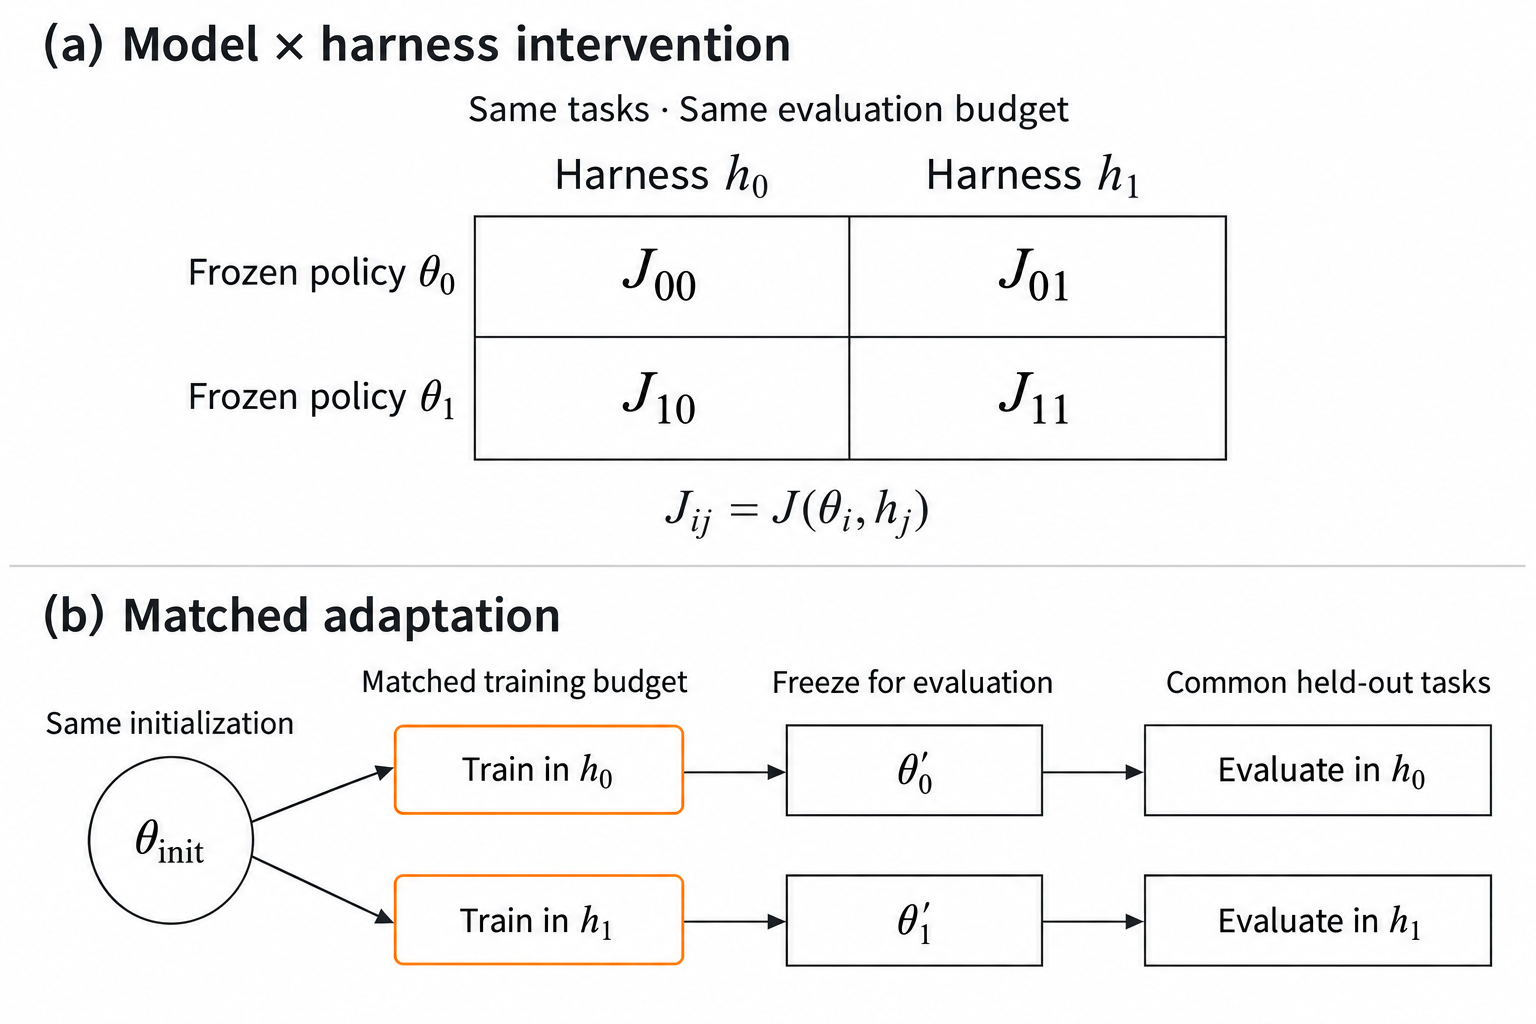
\includegraphics[width=\linewidth]{book/figures/assets/F01bv2.png}
\caption{Two different harness-comparison protocols. (a) $J_{ij}=J(\theta_i,h_j)$ exposes all four fixed-policy cells needed for the interaction in Equation~\ref{eq:C01:interaction}, under common tasks and evaluation limits. Entries are symbolic outcomes, not measurements. (b) Each $\theta_i'$ is obtained from the same $\theta_{\mathrm{init}}$ with matched training budgets before evaluation in $h_i$ on common held-out tasks. Primes denote adapted checkpoints frozen for evaluation, not certified optima. Compatible tasks, grading, and leakage checks remain necessary.}
\label{fig:C01:comparisons}
\end{figure}

